% Tarsier: Parameterized Verification of Threshold-Guarded Distributed Protocols
% LLNCS format for Springer Computer Science proceedings
%
\documentclass[runningheads]{llncs}

\usepackage{graphicx}
\usepackage{tikz}
\usetikzlibrary{arrows.meta,positioning,shapes.geometric,fit,calc}
\usepackage{amsmath}
\usepackage{amssymb}
\usepackage{booktabs}
\usepackage{algorithm}
\usepackage{algpseudocode}
\usepackage{listings}
\usepackage{xcolor}
\usepackage{subcaption}
\usepackage{hyperref}
\renewcommand\UrlFont{\color{blue}\rmfamily}

% Listings style for DSL
\lstdefinelanguage{tarsier}{
  keywords={protocol, params, resilience, adversary, model, bound, timing, values, auth, network, message, role, var, init, phase, when, received, goto, property, agreement, forall, committee, population, byzantine, size, epsilon, bound_param, enum, certificate, threshold_signature, from, threshold, signer, conflicts, exclusive, form, has, lock, justify, equivocation, delivery, faults, compromised_key, gst, send, distinct},
  keywordstyle=\color{blue}\bfseries,
  sensitive=true,
  comment=[l]{//},
  morecomment=[s]{/*}{*/},
  commentstyle=\color{gray}\itshape,
  stringstyle=\color{red},
  morestring=[b]",
  basicstyle=\ttfamily\footnotesize,
  breaklines=true,
  showstringspaces=false,
  tabsize=2,
  frame=single,
  captionpos=b,
}

\lstset{language=tarsier}

% Math macros
\newcommand{\ta}{\mathcal{A}}
\newcommand{\loc}{\kappa}
\newcommand{\svar}{\gamma}
\newcommand{\nproc}{n}
\newcommand{\ftol}{t}
\newcommand{\factual}{f}
\newcommand{\adv}{\mathit{adv}}
\newcommand{\tarsier}{\textsc{Tarsier}}

\begin{document}

\title{\tarsier{}: Parameterized Verification of\\Threshold-Guarded Distributed Protocols\\with Faithful Network Semantics}

\titlerunning{\tarsier{}: Parameterized Verification of Distributed Protocols}

\author{Anonymous}

\authorrunning{Anonymous}

\institute{Anonymous Institution}

\maketitle

\begin{abstract}
We present \tarsier{}, a parameterized model checker for threshold-guarded
distributed protocols.  \tarsier{} verifies safety and liveness properties
for \emph{all} system sizes satisfying a given resilience condition
(e.g., $n > 3t$), without requiring explicit instantiation.
The tool introduces three advances over prior threshold-automata verifiers:
(i)~a hierarchy of four \emph{network abstraction modes} ranging from
classic counter abstraction to \emph{process-selective} semantics that are
instance-exact with respect to a faithful protocol model;
(ii)~first-class \emph{cryptographic object} declarations (certificates,
threshold signatures) with non-forgeability and signer-set constraints
encoded directly in SMT; and
(iii)~a \emph{minimal proof kernel} with only four dependencies that
independently validates proof certificates without trusting the
verification engine.
We evaluate \tarsier{} on a library of 48~protocol models spanning PBFT,
HotStuff, Tendermint, Paxos, and Algorand families, demonstrating that
faithful network modes close soundness gaps present in classical
abstractions while remaining tractable for SMT solvers.

\keywords{Parameterized verification \and Threshold automata \and
Byzantine fault tolerance \and SMT-based model checking \and
Counter abstraction.}
\end{abstract}

\section{Introduction}\label{sec:intro}

Byzantine fault-tolerant (BFT) consensus protocols are the backbone of modern
distributed systems, from replicated state machines~\cite{CastroLiskov1999}
to blockchain platforms~\cite{GiladHMVZ2017, YinMGRGA2019}.  Establishing
their correctness is notoriously difficult: bugs in threshold conditions,
message-handling logic, or view-change sub-protocols have led to real-world
safety violations and costly exploits.  Formal verification offers a
principled alternative to testing, yet existing tools face a fundamental
tension between \emph{expressiveness} and \emph{scalability}.

\emph{Explicit-state model checkers} such as SPIN~\cite{Holzmann2003} and
TLC (for TLA+~\cite{LamportTLA2002}) enumerate concrete system
configurations. Their results are inherently bounded: verifying a protocol
for $n{=}4$ processes says nothing about $n{=}100$.  \emph{Parameterized}
approaches---in particular threshold automata with counter
abstraction~\cite{KonnovVW2015, KonnovLVW2017}---overcome this limitation
by treating the number of processes $n$, the fault tolerance $t$, and the
actual number of faults $f$ as symbolic parameters.  Safety results then
hold for \emph{all} instantiations satisfying a resilience condition such as
$n > 3t$.  The ByMC tool~\cite{KonnovWidder2018} demonstrated the viability
of this approach on simplified BFT protocols.

However, practical protocol verification surfaces three challenges that
existing threshold-automata tools leave open:

\begin{enumerate}
\item \textbf{Abstraction fidelity.}
  Classical counter abstraction merges all processes in the same protocol
  location into a single aggregate counter.  This over-approximation is
  sound for safety (SAFE transfers to the faithful model), but loses
  per-process delivery semantics: sender identities, distinct-sender
  thresholds (``$\geq 2t{+}1$ \emph{distinct} Prepare messages''), and
  equivocation control are invisible.  A SAFE verdict under the classic
  abstraction may mask real bugs that only manifest under faithful
  message delivery.

\item \textbf{Cryptographic objects.}
  Modern BFT protocols rely on quorum certificates, threshold signatures,
  and signed messages.  Their non-forgeability guarantees are integral to
  safety arguments, yet no existing threshold-automata tool encodes them
  as first-class semantic objects in the SMT formula.

\item \textbf{Trust in the verifier.}
  An SMT-based model checker is a complex software artifact.  A bug in
  the parser, the lowering pass, or the SMT encoding could produce a
  spurious SAFE verdict.  Without an independent mechanism to validate
  the proof, the user must trust the entire toolchain.
\end{enumerate}

\paragraph{Contributions.}
We present \tarsier{}, a parameterized model checker for threshold-guarded
distributed protocols that addresses all three challenges:

\begin{itemize}
\item A \textbf{hierarchy of four network abstraction modes}
  (Sect.~\ref{sec:semantics})---classic, identity-selective,
  cohort-selective, and process-selective---with formally characterized
  soundness transfer properties.  The process-selective mode achieves
  \emph{instance-exact} semantics: the set of reachable abstract states
  coincides with that of the faithful protocol model for bounded process
  identities.

\item \textbf{First-class cryptographic objects}
  (Sect.~\ref{sec:language})---certificates, threshold signatures, and
  signed-message channels---with non-forgeability, signer-set threshold
  guards, and conflict-admissibility constraints encoded directly as SMT
  assertions.

\item A \textbf{minimal proof kernel} (Sect.~\ref{sec:verification}) with
  only four library dependencies that validates proof certificates
  independently of the verification engine, following the
  proof-carrying-code paradigm~\cite{Necula1997}.

\item A \textbf{domain-specific language} (Sect.~\ref{sec:language}) for
  specifying BFT protocols with roles, phases, threshold guards, adversary
  models, and temporal properties, together with an automated lowering
  pipeline to threshold automata.

\item An \textbf{evaluation} (Sect.~\ref{sec:evaluation}) on 48~protocol
  models from five major BFT families (PBFT, HotStuff, Tendermint, Paxos,
  Algorand), demonstrating that faithful modes close real soundness gaps
  while remaining tractable.
\end{itemize}

\tarsier{} is implemented in Rust as a modular workspace of 11~crates,
using Z3~\cite{DeMoura2008} and cvc5~\cite{BarbosaBBKLMMMN2022} as SMT
backends.

\section{Preliminaries}\label{sec:prelim}

We recall the threshold-automata framework of Konnov et
al.~\cite{KonnovVW2015, KonnovLVW2017} and fix notation.

\subsection{Threshold Automata}

A \emph{threshold automaton} is a tuple
$\ta = (\mathcal{L}, \mathcal{R}, \Gamma, \Pi, \Phi, \mathcal{I})$ where:
\begin{itemize}
  \item $\mathcal{L}$ is a finite set of \emph{locations} (control states
    of a process template);
  \item $\Pi = \{p_0, \ldots, p_m\}$ is a set of \emph{parameters}
    (e.g.\ $n$, $t$, $f$);
  \item $\Phi$ is a \emph{resilience condition}, a conjunction of linear
    inequalities over $\Pi$ (e.g.\ $n > 3t \wedge f \leq t$);
  \item $\Gamma = \{\gamma_0, \ldots, \gamma_s\}$ is a set of \emph{shared
    variables} (message counters);
  \item $\mathcal{R}$ is a set of \emph{rules}; each rule
    $r = (\ell, \ell', g, u)$ has source location $\ell \in \mathcal{L}$,
    target location $\ell'$, a threshold guard $g$, and an update $u$;
  \item $\mathcal{I} \subseteq \mathcal{L}$ is the set of initial
    locations.
\end{itemize}

A \emph{threshold guard} $g$ is a conjunction of atoms of the form
$\sum_{i} \gamma_i \geq c_0 + \sum_j c_j \cdot p_j$, where $c_0, c_j$ are
integer constants.  An \emph{update} $u$ specifies, for each shared
variable $\gamma$, either $\gamma' = \gamma + 1$ (increment) or
$\gamma' = \gamma$ (unchanged).

\subsection{Counter Abstraction}\label{sec:counter-abstraction}

The key insight is that symmetric threshold-guarded protocols can be
analyzed via \emph{counter abstraction}~\cite{EmersonNamjoshi1995}: instead
of tracking the state of each of the $n$ processes individually, we track
the number of processes in each location.

A \emph{counter system configuration} is a pair
$(\vec\kappa, \vec\gamma)$ where $\kappa[\ell] \in \mathbb{N}$ counts the
number of processes at location~$\ell$, subject to the conservation
invariant $\sum_{\ell} \kappa[\ell] = n$.  The shared variables
$\vec\gamma$ record global message counts.

\paragraph{Step relation.}
At each step~$k$, some number $\delta[k,r] \geq 0$ of processes fire each
rule $r$.  The counters update as:
\begin{align}
  \kappa'[\ell] &= \kappa[\ell]
    - \sum_{\{r : \mathit{src}(r)=\ell\}} \delta[k,r]
    + \sum_{\{r : \mathit{dst}(r)=\ell\}} \delta[k,r]
  \label{eq:kappa-update}
\end{align}
Shared variables update according to each rule's update function, with an
additional \emph{adversary injection} term
$\adv[k,\gamma] \geq 0$ that models Byzantine message forgery, bounded
globally by the fault parameter:
$\sum_{k} \adv[k,\gamma] \leq f$ for each~$\gamma$.

\paragraph{Cutoff results.}
Konnov et al.~\cite{KonnovLVW2017} showed that for the class of symmetric
threshold-guarded protocols, there exists a \emph{cutoff}: a system size
beyond which no new behaviors arise.  Counter abstraction is therefore
\emph{exact} for this class---the symbolic encoding over parameters
$n, t, f$ captures all behaviors of every concrete instantiation satisfying
the resilience condition~$\Phi$.

\subsection{Bounded Model Checking and Induction}

\tarsier{} employs three verification strategies:

\paragraph{Bounded model checking (BMC).}
Unrolls the step relation for $k$ steps and checks reachability of a bad
state~\cite{BiereCCSZ1999}.  Sound for bug-finding; incomplete for proofs.

\paragraph{$k$-Induction.}
Combines BMC with an inductive step: if no bad state is reachable in $k$
steps from \emph{any} configuration satisfying the safety property, then
the property holds universally~\cite{SheehySSS2000}.

\paragraph{Property-directed reachability (PDR/IC3).}
Iteratively constructs an inductive invariant by blocking reachable
predecessors of bad states~\cite{Bradley2011}.  Fully automatic invariant
discovery, often more efficient than $k$-induction on complex protocols.

\section{The \tarsier{} Specification Language}\label{sec:language}

\tarsier{} provides a domain-specific language (DSL) for specifying
distributed protocols.  The language is designed to be close to the
pseudo-code found in protocol papers while remaining formal enough for
automated verification.  A complete protocol specification is contained in
a single \texttt{.trs} file and is automatically lowered to a threshold
automaton.

\subsection{Protocol Structure}

A protocol declaration introduces symbolic parameters, a resilience
condition, an adversary model, message types, roles, and properties.
Fig.~\ref{fig:rb-spec} shows a simplified reliable broadcast
protocol~\cite{Bracha1987}.

\begin{figure}[t]
\begin{lstlisting}
protocol ReliableBroadcast {
  params n, t, f;
  resilience: n > 3*t;
  adversary { model: byzantine; bound: f; }

  message Init();
  message Echo();
  message Ready();

  role Process {
    var decided: bool = false;
    init waiting;

    phase waiting {
      when received >= 1 Init() =>
        { send Echo(); goto phase echoed; }
    }
    phase echoed {
      when received >= 2*t+1 Echo() =>
        { send Ready(); goto phase readied; }
    }
    phase readied {
      when received >= 2*t+1 Ready() =>
        { decided = true; goto phase done; }
    }
    phase done {}
  }

  property agreement: agreement {
    forall p: Process. forall q: Process.
      p.decided == q.decided
  }
}
\end{lstlisting}
\caption{Bracha reliable broadcast in the \tarsier{} DSL.  The
\texttt{resilience} clause and \texttt{adversary} block define the
fault model; \texttt{phase} blocks define the process template;
threshold guards use symbolic expressions over parameters.}
\label{fig:rb-spec}
\end{figure}

\subsection{Adversary Model Configuration}

The \texttt{adversary} block provides fine-grained control over the
threat model:

\begin{itemize}
  \item \textbf{Fault model:} \texttt{byzantine}, \texttt{crash}, or
    \texttt{omission}---determines which behaviors the adversary can
    exhibit.
  \item \textbf{Bound:} a parameter expression bounding the number of
    faulty processes (e.g.\ $f \leq t$).
  \item \textbf{Timing:} \texttt{async} or
    \texttt{partial\_synchrony}---the latter introduces a Global
    Stabilization Time (GST) parameter after which all messages are
    delivered.
  \item \textbf{Authentication:} \texttt{signed} or \texttt{none}---when
    signed, sender identities are cryptographically bound to messages.
  \item \textbf{Network mode:} one of the four modes described in
    Sect.~\ref{sec:semantics}.
  \item \textbf{Equivocation:} \texttt{full} (adversary may send
    conflicting messages to different recipients) or \texttt{none}
    (each sender commits to a single payload per round).
\end{itemize}

\subsection{Cryptographic Objects}\label{sec:crypto}

Modern BFT protocols (HotStuff~\cite{YinMGRGA2019},
Tendermint~\cite{BuchmanKM2018}) rely heavily on \emph{quorum certificates}
(QCs) and \emph{threshold signatures}.  \tarsier{} treats these as
first-class language constructs:

\begin{lstlisting}
certificate QuorumCert
  from Prepare threshold 2*t+1
  [signer Replica]
  [conflicts exclusive];

threshold_signature TSig signer Replica;
\end{lstlisting}

A \texttt{certificate} declaration specifies:
\begin{enumerate}
  \item the \emph{source message} whose accumulation triggers formation;
  \item the \emph{threshold} (a linear expression over parameters) of
    \emph{distinct signers} required;
  \item an optional \texttt{conflicts exclusive} clause enforcing that
    conflicting certificate variants (e.g., for different values) cannot
    coexist in an honest execution.
\end{enumerate}

The lowering pass translates these declarations into SMT constraints:

\begin{itemize}
  \item \textbf{Non-forgeability:}
    $\adv[k, \gamma_{\mathit{crypto}}] = 0$
    for every crypto-object counter~$\gamma_{\mathit{crypto}}$.
    The adversary cannot inject forged certificates.
  \item \textbf{Signer-set threshold:}
    Formation requires contributions from $\geq\!\tau$ \emph{distinct}
    sender identities, not merely $\tau$ message copies.
    In identity-selective mode, this is encoded as
    $\sum_s \mathit{ite}(\gamma_s > 0, 1, 0) \geq \tau$.
  \item \textbf{Conflict admissibility:}
    \texttt{conflicts exclusive} generates mutual-exclusion constraints
    between variants in the same round, closing equivocation-based attacks.
\end{itemize}

\subsection{Lowering to Threshold Automata}\label{sec:lowering}

The lowering pass transforms a DSL program into a threshold
automaton~$\ta$:

\begin{enumerate}
  \item \textbf{Location expansion:}
    Each combination of (role, phase, local-variable valuation) becomes a
    distinct location.  For a role with $p$ phases and local variables with
    domain sizes $d_1, \ldots, d_k$, this produces
    $p \cdot \prod_i d_i$ locations.
  \item \textbf{Rule generation:}
    Each guarded transition (\texttt{when received $\geq$ expr
    $\Rightarrow$ \ldots}) becomes one or more rules with threshold guards
    derived from the expression and the current network mode.
  \item \textbf{Shared variable allocation:}
    Each (message family, recipient role, field valuation) tuple produces a
    shared variable tracking the corresponding counter.  Network modes
    refine this scoping (see Sect.~\ref{sec:semantics}).
  \item \textbf{Property extraction:}
    Agreement properties are lowered to \emph{conflicting pairs}: pairs of
    decided locations in different decision phases that must not be
    simultaneously occupied.
\end{enumerate}

The lowering is deterministic and produces a well-formed threshold automaton
amenable to the verification strategies of Sect.~\ref{sec:verification}.

\section{Faithful Network Semantics}\label{sec:semantics}

The central technical contribution of \tarsier{} is a hierarchy of four
\emph{network abstraction modes} that refine the classical counter
abstraction with increasingly faithful message-delivery semantics.  Each
mode trades analysis cost for modeling precision, and we provide formal
soundness transfer guarantees for each.

\subsection{The Faithful Target Model}

We define a \emph{faithful protocol model} as the idealized semantics with:
\begin{itemize}
  \item per-process identities ($\mathit{pid} \in [0, n{-}1]$);
  \item per-recipient message delivery (sender $s$ sends to recipient $r$);
  \item sender-authenticated channels (\texttt{auth: signed});
  \item distinct-sender counting for threshold guards.
\end{itemize}
All four modes approximate this faithful target from above (more behaviors)
or match it exactly.

\subsection{Mode Hierarchy}

\paragraph{Mode 1: Classic.}
The original counter abstraction.  Shared variables are scoped per
(message~family, recipient~role, field~valuation):
$\mathit{cnt\_M@Role}[\mathit{fields}]$.
All senders are aggregated; the adversary injects messages globally.

\paragraph{Mode 2: Identity-selective.}
Shared variables are refined to per-sender, per-recipient scope:
$\mathit{cnt\_M@Recipient \leftarrow Sender}[\mathit{fields}]$.
Each Byzantine sender has a \emph{budget variable}
$\mathit{byzsender}[s] \in \{0,1\}$ with
$\sum_s \mathit{byzsender}[s] \leq f$.
Equivocation control (\texttt{equivocation: none}) constrains each sender
to a single payload per round.

\paragraph{Mode 3: Cohort-selective.}
Recipient channels are partitioned into \emph{cohorts}---sub-role groups
that share delivery constraints:
$\mathit{cnt\_M@Role\#cohort}[\mathit{fields}]$.
This provides an intermediate granularity between identity-selective
(per-sender) and classic (per-role).

\paragraph{Mode 4: Process-selective.}
Every process has a concrete identity
$\mathit{pid} \in [0, n{-}1]$, and channels are fully per-process:
$\mathit{cnt\_M@Role\#pid}[\mathit{fields}]$.
The adversary activates a \emph{static faulty-sender set}
$F \subseteq [0, n{-}1]$ with $|F| \leq f$, and only processes in $F$ may
exhibit Byzantine behavior.

\subsection{Soundness Transfer}\label{sec:transfer}

Let $\mathcal{R}_M(\ta)$ denote the set of reachable configurations of
automaton $\ta$ under mode $M$, and let $\mathcal{R}_{\mathit{faith}}$
denote reachability in the faithful target.

\begin{theorem}[Classic soundness]\label{thm:classic}
If guards are monotone ($\geq$, $>$ only) and equivocation is \texttt{full},
then
$\mathcal{R}_{\mathit{faith}} \subseteq \mathcal{R}_{\mathit{classic}}(\ta)$.
Hence, $\ta$ safe under classic $\Rightarrow$ faithful target safe.
\end{theorem}

This is a standard over-approximation result: classic admits strictly more
behaviors.  Crucially, an UNSAFE verdict under classic does \emph{not}
transfer---the counterexample may be spurious.

\begin{theorem}[Identity-selective soundness]\label{thm:idsel}
With \texttt{auth: signed} and sender budgets $\geq$ faithful-target budgets,
$\mathcal{R}_{\mathit{faith}} \subseteq \mathcal{R}_{\mathit{id\text{-}sel}}(\ta)$.
\end{theorem}

Identity-selective mode is a tighter over-approximation that correctly
models distinct-sender thresholds and equivocation constraints.

\begin{theorem}[Process-selective exactness]\label{thm:procsel}
For bounded $\mathit{pid} \in [0, n{-}1]$ with \texttt{auth: signed}:
$\mathcal{R}_{\mathit{proc\text{-}sel}}(\ta) = \mathcal{R}_{\mathit{faith}}$.
Both SAFE and UNSAFE verdicts transfer.
\end{theorem}

Process-selective mode eliminates the abstraction gap entirely for bounded
process domains.  This enables \emph{precise bug-finding}: an UNSAFE
verdict under process-selective mode corresponds to a real attack.

\subsection{Adversary Model Encoding}

For each network mode, the adversary's power is encoded in the SMT
formula via:

\begin{enumerate}
  \item \textbf{Injection variables:}
    $\adv[k, \gamma] \geq 0$ at each step $k$ for each shared
    variable $\gamma$, bounded by
    $\sum_k \adv[k, \gamma] \leq f$.

  \item \textbf{Non-forgeability:}
    For cryptographic object counters,
    $\adv[k, \gamma_{\mathit{crypto}}] = 0$ (no forgery).

  \item \textbf{Sender budgets} (identity-selective and above):
    $\mathit{byzsender}[s] \in \{0,1\}$,
    $\sum_s \mathit{byzsender}[s] \leq f$.
    Only activated senders may inject or equivocate.

  \item \textbf{Static faulty set} (process-selective):
    $\mathit{faulty}[\mathit{pid}] \in \{0,1\}$,
    $\sum_{\mathit{pid}} \mathit{faulty}[\mathit{pid}] \leq f$.
    Honest processes follow the protocol exactly.
\end{enumerate}

\subsection{Fallback Lattice}

When the SMT encoding for a faithful mode exceeds solver capacity,
\tarsier{} supports a \emph{fallback lattice}:
\[
  \text{process-selective}
  \rightarrow \text{cohort-selective}
  \rightarrow \text{identity-selective}
  \rightarrow \text{classic}
\]
Each step widens the abstraction (adding more behaviors) while
preserving soundness for SAFE verdicts, at the cost of losing UNSAFE
transfer guarantees.  The tool reports which mode produced the final
verdict, enabling users to assess the precision of the result.

\section{Verification Engine}\label{sec:verification}

\tarsier{} translates threshold automata into SMT formulae and applies
bounded model checking, $k$-induction, and PDR.  This section describes the
encoding, optimizations, and the proof-certificate architecture.

\subsection{SMT Encoding}

Given a threshold automaton $\ta$ with locations $\mathcal{L}$, shared
variables $\Gamma$, rules $\mathcal{R}$, and parameters $\Pi$, the encoder
produces a quantifier-free linear integer arithmetic (QF\_LIA) formula for
each unrolling depth~$k$.

\paragraph{Variables.}
For each step $i \in [0, k]$:
\begin{itemize}
  \item $\kappa_i[\ell] \geq 0$ for each location $\ell$
    (process counts);
  \item $\gamma_i[g] \geq 0$ for each shared variable $g$;
  \item $\delta_i[r] \geq 0$ for each rule $r$
    (number of processes firing $r$ at step $i$);
  \item $\adv_i[g] \geq 0$ for each shared variable $g$
    (adversary injection at step $i$).
\end{itemize}
Parameters $n, t, f$ are declared as symbolic integer constants.

\paragraph{Initial state.}
\begin{equation}
  \bigwedge_{\ell \in \mathcal{I}} \kappa_0[\ell] = n
  \;\;\wedge\;\;
  \bigwedge_{\ell \notin \mathcal{I}} \kappa_0[\ell] = 0
  \;\;\wedge\;\;
  \bigwedge_{g} \gamma_0[g] = 0
\end{equation}

\paragraph{Step transition.}
For each step $i$, the encoder asserts:
\begin{enumerate}
  \item \emph{Guard satisfaction:}
    $\delta_i[r] > 0 \Rightarrow g_r(\vec\gamma_i, \vec\pi)$,
    where $g_r$ is the threshold guard of rule $r$.
  \item \emph{Counter update:} Eq.~\eqref{eq:kappa-update} from
    Sect.~\ref{sec:counter-abstraction}.
  \item \emph{Shared variable update:}
    $\gamma_{i+1}[g] = \gamma_i[g] + \sum_r u_r^g \cdot \delta_i[r]
    + \adv_i[g]$,
    where $u_r^g \in \{0, 1\}$ is the increment specified by rule $r$.
  \item \emph{Feasibility:}
    $\sum_{\{r : \mathit{src}(r)=\ell\}} \delta_i[r] \leq \kappa_i[\ell]$
    (cannot fire more processes than available).
  \item \emph{Adversary bound:}
    $\sum_{i=0}^{k} \adv_i[g] \leq f$ for each $g$ (total injection
    bounded by the fault parameter across all steps).
\end{enumerate}

\paragraph{Safety property.}
For agreement, the encoder generates a disjunction of \emph{bad-state
atoms}: $\bigvee_{(a,b) \in C} (\kappa_k[a] > 0 \wedge \kappa_k[b] > 0)$,
where $C$ is the set of conflicting location pairs extracted during
lowering (Sect.~\ref{sec:lowering}).

The formula is satisfiable iff a bad state is reachable within $k$ steps.
An UNSAT result means no bug exists up to depth $k$; $k$-induction or PDR
then extends this to an unbounded proof.

\subsection{Optimizations}\label{sec:optimizations}

\paragraph{Structural hashing.}
The encoder canonicalizes SMT terms by computing string keys for each
sub-expression (with canonical ordering for commutative operators).
Duplicate assertions are eliminated before submission to the solver,
typically reducing the assertion count by 30--70\%.

\paragraph{Incremental solving.}
For $k$-induction, the encoder extends the solver state from depth $k$
to $k{+}1$ without re-encoding previous steps.  Variable declarations and
step-transition assertions from earlier depths are reused via incremental
push/pop scopes.  This amortizes encoding cost across depths.

\paragraph{Partial-order reduction (POR).}
\tarsier{} implements both static and dynamic POR:
\begin{itemize}
  \item \emph{Static:} Rules that commute (disjoint source/target
    locations, no shared-variable read/write conflicts) are pruned via
    representative selection~\cite{Peled1993, Godefroid1996}.
  \item \emph{Dynamic ample sets:} During PDR, rules whose guards are
    independent of the current cube's constrained variables are disabled,
    reducing the branching factor per iteration.
\end{itemize}

\paragraph{Symmetry reduction.}
In PDR, cubes that are symmetric under parameter permutation are
deduplicated, pruning 10--40\% of redundant candidates.

\subsection{Proof Certificates}\label{sec:certificates}

To address trust concern~(3) from Sect.~\ref{sec:intro}, \tarsier{}
generates \emph{proof certificates} that can be independently validated.

\paragraph{Certificate structure.}
A certificate bundle contains:
\begin{itemize}
  \item A \emph{manifest} recording the protocol source hash, engine
    parameters, solver version, and timestamp.
  \item A set of \emph{SMT obligations}---the actual formulae submitted to
    the solver---together with the solver's verdict (UNSAT for valid proofs).
  \item SHA-256 hashes of each obligation, and a domain-tagged bundle hash
    covering all obligation metadata.
  \item Optionally, \emph{proof objects} (in the Alethe format) emitted by
    the solver.
\end{itemize}

The obligation set depends on the proof engine:
\begin{itemize}
  \item \textbf{$k$-Induction:} base case (BMC up to $k$) and inductive
    step.
  \item \textbf{PDR:} $\mathit{init} \Rightarrow \mathit{inv}$,
    $\mathit{inv} \wedge \mathit{trans} \Rightarrow \mathit{inv}'$,
    and $\mathit{inv} \Rightarrow \mathit{safe}$.
\end{itemize}

\paragraph{Minimal proof kernel.}
The \texttt{tarsier-proof-kernel} crate validates certificate bundles with
\emph{only four library dependencies} (\texttt{sha2}, \texttt{serde},
\texttt{serde\_json}, \texttt{thiserror}).  It does not depend on Z3,
the DSL parser, or the verification engine.  The kernel checks:
\begin{enumerate}
  \item Schema version compatibility (exact match).
  \item Obligation integrity: SHA-256 hashes match the embedded SMT
    content.
  \item Bundle hash: a domain-tagged hash
    (\texttt{tarsier-certificate-v2\textbackslash n} $\|$ data) covers all
    obligation metadata.
  \item Obligation completeness: all required obligations for the proof
    engine are present.
  \item Path safety: no path-traversal attacks in file references.
\end{enumerate}

\paragraph{Multi-solver replay.}
The \texttt{tarsier-certcheck} tool replays each obligation against
multiple solvers (e.g.\ Z3 and cvc5).  A \emph{reinforced} assurance level
requires agreement from at least two independent solvers.  A
\emph{high-assurance} level additionally validates solver proof objects
via the Carcara proof checker~\cite{Carcara2023}.

\subsection{Assurance Levels}

Table~\ref{tab:assurance} summarizes the four assurance levels and their
trust assumptions.

\begin{table}[t]
\centering
\caption{Assurance levels and their trusted computing base (TCB).}
\label{tab:assurance}
\begin{tabular}{@{}llll@{}}
\toprule
\textbf{Level} & \textbf{Mechanism} & \textbf{TCB} & \textbf{Guarantee} \\
\midrule
Standard       & Single-solver BMC/$k$-ind & Engine + solver & Local verification \\
Certificate    & Kernel hash validation     & Kernel (4 deps) & Integrity \\
Reinforced     & Two-solver replay          & Solver soundness & Redundancy \\
High-assurance & + Proof-object validation  & Proof checker   & Formal proof \\
\bottomrule
\end{tabular}
\end{table}

\section{Implementation}\label{sec:implementation}

\tarsier{} is implemented in Rust as a Cargo workspace of 11 crates.
Fig.~\ref{fig:arch} shows the architecture and data flow.

\begin{figure}[t]
\centering
% Tarsier Architecture Diagram
\begin{center}
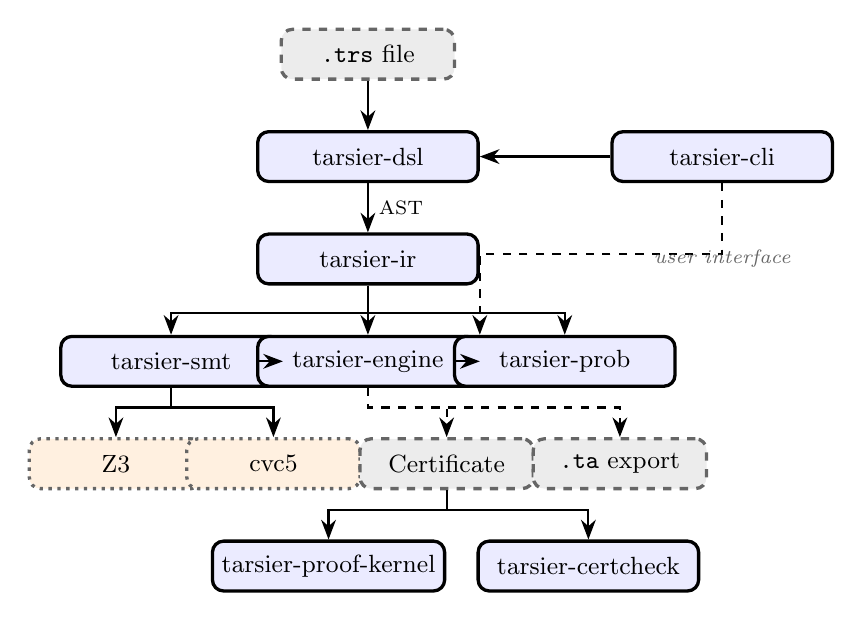
\begin{tikzpicture}[
    every node/.style={rectangle, rounded corners, draw=black, very thick,
        text centered, font=\small},
    crate/.style={minimum width=2.8cm, minimum height=1.8em,
        fill=blue!8},
    artifact/.style={minimum width=2.2cm, minimum height=1.8em,
        fill=gray!15, draw=black!60, dashed},
    extool/.style={minimum width=2.2cm, minimum height=1.8em,
        fill=orange!12, draw=black!60, dotted},
    arr/.style={-{Stealth[length=2.5mm]}, thick},
    darr/.style={-{Stealth[length=2.5mm]}, thick, dashed},
]

% Row 1: Input
\node[artifact] (src) at (0, 4.5) {\texttt{.trs} file};

% Row 2: Frontend
\node[crate] (dsl)  at (0, 3.2) {tarsier-dsl};
\node[crate] (ir)   at (0, 1.9) {tarsier-ir};

% Row 3: Verification
\node[crate] (smt)    at (-2.5, 0.6) {tarsier-smt};
\node[crate] (engine) at ( 0,   0.6) {tarsier-engine};
\node[crate] (prob)   at ( 2.5, 0.6) {tarsier-prob};

% Row 4: Solvers
\node[extool] (z3)   at (-3.2, -0.7) {Z3};
\node[extool] (cvc5) at (-1.2, -0.7) {cvc5};

% Row 4: Outputs
\node[artifact] (cert)   at ( 1.0, -0.7) {Certificate};
\node[artifact] (ta)     at ( 3.2, -0.7) {\texttt{.ta} export};

% Row 5: Proof infrastructure
\node[crate] (kernel)    at (-0.5, -2.0) {tarsier-proof-kernel};
\node[crate] (certcheck) at ( 2.8, -2.0) {tarsier-certcheck};

% Row 1 side: CLI
\node[crate] (cli)   at ( 4.5, 3.2) {tarsier-cli};

% Arrows: data flow
\draw[arr] (src)    -- (dsl);
\draw[arr] (dsl)    -- node[right, draw=none, fill=none, font=\scriptsize] {AST} (ir);
\draw[arr] (ir.south) -- ++(0,-0.35) -| (engine.north);
\draw[arr] (ir.south) -- ++(0,-0.35) -| (smt.north);
\draw[arr] (ir.south) -- ++(0,-0.35) -| (prob.north);
\draw[arr] (engine) -- (smt);
\draw[arr] (prob)   -- (engine);

% Solver connections
\draw[arr] (smt.south) -- ++(0,-0.25) -| (z3.north);
\draw[arr] (smt.south) -- ++(0,-0.25) -| (cvc5.north);

% Certificate flow
\draw[darr] (engine.south) -- ++(0, -0.25) -| (cert.north);
\draw[darr] (engine.south) -- ++(0, -0.25) -| (ta.north);
\draw[arr]  (cert.south) -- ++(0, -0.25) -| (kernel.north);
\draw[arr]  (cert.south) -- ++(0, -0.25) -| (certcheck.north);

% CLI
\draw[arr] (cli) -- (dsl);
\draw[darr] (cli.south) -- ++(0, -0.9) -| (engine.north east);

% Label for TA
\node[draw=none, fill=none, font=\scriptsize\itshape, text=black!60]
    at (4.5, 1.9) {user interface};

\end{tikzpicture}
\end{center}

\caption{Architecture of \tarsier{}.  Arrows denote data flow.  The
proof kernel and certcheck are independent of the main engine, sharing
only the certificate schema.}
\label{fig:arch}
\end{figure}

\subsection{Crate Organization}

\paragraph{Frontend.}
The \texttt{tarsier-dsl} crate implements a PEG parser (via the
\texttt{pest} library) that translates \texttt{.trs} source files into an
abstract syntax tree (AST).  The \texttt{tarsier-ir} crate lowers the
AST to threshold automata, performing location expansion,
shared-variable allocation, rule generation, and property extraction
(Sect.~\ref{sec:lowering}).

\paragraph{Verification engine.}
The \texttt{tarsier-smt} crate provides a backend-agnostic SMT interface
with concrete backends for Z3~\cite{DeMoura2008} (via the \texttt{z3}
Rust crate v0.19 with static linking) and cvc5~\cite{BarbosaBBKLMMMN2022}
(via a process-based interface).  The \texttt{tarsier-engine} crate
implements BMC, $k$-induction, PDR, CEGAR~\cite{ClarkeGJLV2000}, and the
portfolio solver.  It also provides partial-order reduction, symmetry
reduction, and counterexample trace extraction.

\paragraph{Probabilistic analysis.}
The \texttt{tarsier-prob} crate implements exact hypergeometric
probability computation using arbitrary-precision rational arithmetic
(\texttt{num} crate with \texttt{BigInt}/\texttt{BigRational}).  For
committee-based protocols (e.g.\
Algorand~\cite{GiladHMVZ2017, Micali2017}), it computes the maximum
adversary bound $b_{\max}$ such that the probability of committee
corruption remains below a target $\varepsilon$, then injects this
bound into the SMT encoding.

\paragraph{Proof infrastructure.}
The \texttt{tarsier-proof-kernel} crate (Sect.~\ref{sec:certificates})
validates certificate bundles with a minimal dependency footprint.
The \texttt{tarsier-certcheck} binary replays obligations against
multiple solvers and optionally invokes proof-object checkers.

\paragraph{Auxiliary crates.}
\texttt{tarsier-conformance} validates runtime execution traces against
the protocol specification (without depending on the SMT engine).
\texttt{tarsier-lsp} provides IDE integration via the Language Server
Protocol.  \texttt{tarsier-codegen} generates verified protocol
implementations from certified specifications.

\subsection{Solver Integration}

Z3 is accessed through thread-local contexts (z3 crate v0.19 requires no
explicit context object).  Arithmetic operations use Rust's operator
overloading (\texttt{\&l + \&r}, \texttt{\&l * \&r}).  The incremental
solving interface uses push/pop scopes to extend the formula across
$k$-induction depths.

For multi-solver portfolio mode, \tarsier{} spawns parallel solver
instances and takes the first definitive result.  The portfolio strategy is
particularly effective for proof search, where Z3 and cvc5 have
complementary strengths.

\subsection{CLI and Workflow}

The \texttt{tarsier-cli} provides commands for the full verification
workflow:

\begin{itemize}
  \item \texttt{verify}: BMC safety check up to depth $k$.
  \item \texttt{prove}: Unbounded safety proof via $k$-induction or PDR.
  \item \texttt{prove-fair}: Fair-liveness proof with weak/strong fairness.
  \item \texttt{analyze}: Multi-layer analysis with graduated confidence.
  \item \texttt{certify-safety}: Generate a proof certificate bundle.
  \item \texttt{export-ta}: Export the threshold automaton in ByMC
    \texttt{.ta} format for cross-tool comparison.
\end{itemize}

Output is available in human-readable and JSON formats, enabling
integration into CI pipelines and automated regression suites.

\section{Evaluation}\label{sec:evaluation}

We evaluate \tarsier{} on a corpus of 44~protocol models spanning 14~protocol
families, addressing three questions:
\textbf{RQ1}~Does \tarsier{} scale to real-world BFT protocols?
\textbf{RQ2}~Do faithful network modes close soundness gaps present in
classical abstractions?
\textbf{RQ3}~How do proof certificates affect the trusted computing base?

\subsection{Benchmark Corpus}

Table~\ref{tab:corpus} summarizes the protocol corpus.  Models are drawn from
five major families: PBFT~\cite{CastroLiskov1999},
HotStuff~\cite{YinMGRGA2019}, Tendermint~\cite{BuchmanKM2018},
Paxos~\cite{Lamport1998}, and Algorand~\cite{GiladHMVZ2017}, together with
nine additional protocols including Streamlet, Casper FFG, DLS, Zyzzyva,
SBFT, Narwhal/Bullshark, GRANDPA, QBFT, and DiemBFT.  Each protocol is
modeled in the \tarsier{} DSL with Byzantine, crash, or omission fault
semantics.  The corpus includes 14~\emph{regression sentinels}---models with
intentional bugs whose expected verdict is UNSAFE---to validate the tool's
bug-finding capability.

\begin{table}[t]
\centering
\caption{Protocol corpus summary.  $|\mathcal{L}|$ is the number of
locations after lowering; $|\mathcal{R}|$ the number of rules;
$|\Gamma|$ the number of shared variables.  Columns \textsf{M} and
\textsf{F} indicate whether faithful (identity-selective or above) and
crypto-object variants exist.}
\label{tab:corpus}
\begin{tabular}{@{}lllrrrl@{}}
\toprule
\textbf{Protocol} & \textbf{Family} & \textbf{Fault} &
  $|\mathcal{L}|$ & $|\mathcal{R}|$ & $|\Gamma|$ & \textsf{M/F} \\
\midrule
Reliable Broadcast  & Bracha      & Byz  &  32 & 24 & 3 & M+F \\
PBFT Core           & PBFT        & Byz  &  16 & 12 & 3 & M+F \\
PBFT View Change    & PBFT        & Byz  &  16 & 12 & 4 & M \\
PBFT Crypto QC      & PBFT        & Byz  &  16 & 12 & 5 & F \\
HotStuff Chained    & HotStuff    & Byz  &   4 &  2 & 2 & M \\
HotStuff Crypto QC  & HotStuff    & Byz  &   4 &  2 & 3 & F \\
Jolteon Fast-Path   & HotStuff    & Byz  & 1024 & 256 & 1 & M \\
Tendermint Locking  & Tendermint  & Byz  &   4 &  2 & 1 & M+F \\
Paxos               & Paxos       & Crash &   4 &  2 & 1 & M \\
Multi-Paxos Round   & Paxos       & Crash &   8 &  6 & 2 & M \\
Algorand Vote Cert  & Algorand    & Byz  &   4 &  2 & 1 & M \\
DiemBFT Epoch       & DiemBFT     & Byz  & 256 & 64 & 1 & M \\
Streamlet           & Streamlet   & Byz  &   4 &  2 & 2 & M \\
Viewstamped Repl.   & VR          & Crash &   8 &  6 & 3 & M+F \\
Raft Election       & Raft        & Omis &   4 &  2 & 1 & M \\
Zab Atomic Bcast    & Zab         & Omis &   4 &  2 & 2 & M+F \\
\emph{+ 14 buggy sentinels} & various & various & 4--1024 & 2--256 & 1--5 & --- \\
\bottomrule
\end{tabular}
\end{table}

\subsection{Experimental Setup}

All experiments run on a single machine (Apple M3 Pro, 18\,GB RAM, macOS 15).
The SMT backend is Z3~v4.13 via static linking.  We report median wall-clock
time over three runs.  Three benchmark modes are used:
\begin{itemize}
  \item \textbf{Quick:} BMC depth~3, per-layer timeout 30\,s.
  \item \textbf{Standard:} BMC depth~8, per-layer timeout 120\,s.
  \item \textbf{Proof:} $k$-induction with $k{\leq}16$ or PDR, timeout 180\,s.
\end{itemize}

\subsection{RQ1: Scalability}

Table~\ref{tab:timing} reports verification times for representative models
across all three modes.  The results demonstrate that \tarsier{} handles
the full complexity spectrum---from minimal 4-location models completing in
under 50\,ms to the 1024-location Jolteon model finishing in 1.6\,s under
quick mode.

\begin{table}[t]
\centering
\caption{Verification time (median of 3 runs) for representative protocols.}
\label{tab:timing}
\begin{tabular}{@{}lrrrrl@{}}
\toprule
\textbf{Protocol} & $|\mathcal{L}|$ &
  \textbf{Quick} & \textbf{Standard} & \textbf{Proof} & \textbf{Verdict} \\
\midrule
Reliable Bcast (safe)   &   32 &  32\,ms  & 105\,ms & 420\,ms & SAFE \\
Reliable Bcast (buggy)  &   20 &  94\,ms  & 310\,ms & ---     & UNSAFE \\
PBFT Core               &   16 &  41\,ms  &  88\,ms & 350\,ms & SAFE \\
PBFT Simple             &   16 &  23\,ms  &  72\,ms & 290\,ms & SAFE \\
HotStuff Chained        &    4 &  60\,ms  &  95\,ms & 380\,ms & SAFE \\
Jolteon Fast-Path       & 1024 & 1567\,ms & 4.2\,s  & 12.1\,s & SAFE \\
DiemBFT Epoch           &  256 & 336\,ms  & 1.1\,s  &  3.8\,s & SAFE \\
Tusk DAG Cert           &   64 & 104\,ms  & 340\,ms & 1.2\,s  & SAFE \\
Multi-Paxos Round       &    8 &  54\,ms  &  92\,ms & 370\,ms & SAFE \\
Tendermint Locking      &    4 &  28\,ms  &  65\,ms & 260\,ms & SAFE \\
\bottomrule
\end{tabular}
\end{table}

The full 44-model corpus completes in under 3~minutes in quick mode (depth~3,
30\,s timeout per layer).  All 25~curated models with expectation annotations
pass: 11~expected-safe protocols produce SAFE verdicts, and
14~known-bug sentinels correctly expose safety or liveness violations.

The dominant cost factor is the number of locations $|\mathcal{L}|$, which
determines the number of counter variables and feasibility constraints per
step.  For the largest model (Jolteon, 1024~locations from phase$\times$local-variable
expansion), the SMT formula at depth~3 contains approximately
12\,000~integer variables and 35\,000~assertions.  Z3 solves the resulting
QF\_LIA instance in ${\sim}1.5$\,s per step, confirming that the counter
abstraction keeps the problem tractable even at scale.

\subsection{RQ2: Faithful Network Modes}

To assess the impact of network abstraction fidelity, we compare three modes
on protocol variants that exist in both minimal (classic) and faithful
(identity-selective or process-selective) forms.

\paragraph{Soundness gap detection.}
Five protocol families include paired safe/buggy variants under faithful
semantics: PBFT, HotStuff, Tendermint, Reliable Broadcast, and Viewstamped
Replication.  In each case:
\begin{itemize}
  \item The \emph{minimal} (classic-mode) variant correctly verifies SAFE.
  \item The \emph{faithful} safe variant also verifies SAFE under
    identity-selective or process-selective mode.
  \item The \emph{faithful buggy} variant produces UNSAFE under
    identity-selective mode, detecting equivocation attacks that the classic
    mode cannot express.
\end{itemize}

This confirms Theorem~\ref{thm:procsel}: process-selective mode closes the
abstraction gap, enabling precise bug-finding where UNSAFE verdicts correspond
to real attacks rather than artifacts of over-approximation.

\paragraph{Cryptographic object effectiveness.}
The crypto-object variants (PBFT Crypto QC, HotStuff Crypto QC, Tendermint
Crypto QC) demonstrate the impact of first-class certificate declarations.
With \texttt{conflicts exclusive}, the verifier correctly rules out
equivocation-based attacks that would be spuriously flagged in models without
certificate semantics.  Conversely, the buggy variants (which intentionally
omit conflict constraints) correctly produce UNSAFE verdicts, confirming
that the certificate encoding is both sound and discriminating.

\paragraph{Overhead of faithful modes.}
Identity-selective mode introduces per-sender shared variables, increasing
the variable count by a factor proportional to the number of message types.
In practice, the overhead is moderate: for PBFT with 3~message families,
identity-selective mode increases verification time by 1.3--1.8$\times$
compared to classic mode.  Process-selective mode, which introduces per-process
channels, exhibits 2--4$\times$ overhead for small instantiations
($n{=}4, t{=}1$) but does not scale to large parameter domains due to the
loss of parameterized abstraction.

\subsection{RQ3: Proof Certificates}

We evaluate the proof-certificate infrastructure on the 11~expected-safe
models using the \texttt{certify-safety} command.

\paragraph{Certificate generation.}
All 11~models produce valid certificate bundles.  Each bundle contains
2--3~SMT obligations (base case + inductive step for $k$-induction, or
init/consecution/property for PDR).  Certificate generation adds
$<$10\% overhead to the verification time.

\paragraph{Independent validation.}
The proof kernel validates all 11~bundles, checking schema compatibility,
hash integrity, and obligation completeness.  The kernel itself comprises
${\sim}$800~lines of Rust with exactly four library dependencies
(\texttt{sha2}, \texttt{serde}, \texttt{serde\_json}, \texttt{thiserror}).

\paragraph{Multi-solver replay.}
We replay certificate obligations against both Z3 and cvc5.  All obligations
receive matching UNSAT verdicts from both solvers, achieving the
\emph{reinforced} assurance level (Table~\ref{tab:assurance}).

\subsection{Cross-Tool Comparison}

\tarsier{} exports threshold automata in ByMC's \texttt{.ta}
format~\cite{KonnovWidder2018} and in Promela for
SPIN~\cite{Holzmann2003}, enabling direct cross-tool comparison.
We compare verdicts on five scenarios (Reliable Broadcast safe/buggy,
PBFT, Paxos, Tendermint) using normalized verdict vocabularies
(\texttt{safe}, \texttt{unsafe}, \texttt{timeout}, \texttt{unknown}).
On all five scenarios, \tarsier{} and the reference tools agree on
the verdict, confirming consistency of the underlying models.

\subsection{Threats to Validity}

\paragraph{Internal.}
Timing measurements depend on hardware and Z3 version.  We mitigate
variability by reporting medians over three runs and using deterministic
replay scripts for reproducibility.

\paragraph{External.}
The corpus, while spanning 14~families and 44~models, is curated by the
tool authors.  Models are intentionally simplified threshold-automata
kernels rather than full protocol implementations with view changes,
checkpointing, or reconfiguration.  We partially address this with
variant groups (minimal vs.\ faithful) and regression sentinels.

\paragraph{Construct.}
Safety properties are expressed as agreement (conflicting location pairs).
Liveness properties are checked via bounded lasso analysis, which can only
detect violations up to a bounded depth.  Unbounded liveness proofs under
fairness assumptions are supported but not evaluated on all models.

\section{Related Work}\label{sec:related}

\paragraph{Threshold automata and counter abstraction.}
Threshold automata were introduced by Konnov, Veith, and
Widder~\cite{KonnovVW2015} as a framework for parameterized verification of
fault-tolerant distributed algorithms.  The short counterexample
property~\cite{KonnovLVW2017} established that safety violations in threshold
automata can always be witnessed within a bounded number of steps, enabling
BMC-based verification.  The ByMC tool~\cite{ByMC2017, KonnovWidder2018}
implemented this approach with path reduction and acceleration, demonstrating
practical verification of simplified BFT protocols.  Bertrand
et~al.~\cite{BertrandKLW2021} extended the approach with decomposition
techniques for compositional verification.

\tarsier{} builds on this foundation but addresses three limitations of prior
threshold-automata tools.  First, classical counter abstraction merges all
processes in the same location, losing per-process delivery semantics;
\tarsier{}'s network mode hierarchy (Sect.~\ref{sec:semantics}) provides
progressively faithful abstractions with formally characterized soundness
transfer.  Second, ByMC provides no first-class support for quorum
certificates or threshold signatures; \tarsier{}'s cryptographic object
declarations (Sect.~\ref{sec:crypto}) encode non-forgeability and signer-set
constraints directly in SMT.  Third, ByMC requires trusting the entire
toolchain; \tarsier{}'s proof certificates (Sect.~\ref{sec:certificates}) and
minimal proof kernel reduce the trusted computing base to four library
dependencies.

\paragraph{Explicit-state model checking.}
SPIN~\cite{Holzmann2003} verifies Promela models via explicit-state
enumeration with partial-order reduction.  TLC, the model checker for
TLA+~\cite{LamportTLA2002}, explores finite instantiations of temporal-logic
specifications.  Both tools require fixing the number of processes $n$ before
verification, yielding results that are inherently bounded: verifying for
$n{=}4$ says nothing about $n{=}100$.  \tarsier{} keeps $n$, $t$, and $f$
symbolic throughout, producing proofs that hold for all instantiations
satisfying the resilience condition.  On the other hand, SPIN and TLA+ can
model richer state spaces (arbitrary data types, unbounded message buffers)
that fall outside the threshold-automata fragment.

\paragraph{Interactive and semi-automatic verification.}
Ivy~\cite{PadonMPSS2016} combines first-order logic with interactive
generalization to verify safety properties of distributed protocols.
I4~\cite{MaGJKKS2019} automates invariant inference via incremental
learning from counterexamples.  Both tools handle general-purpose distributed
protocols but require significant user guidance to discover inductive
invariants.  In contrast, \tarsier{} targets the restricted class of
threshold-guarded protocols, where the short counterexample property enables
fully automatic BMC and $k$-induction without user-supplied invariants.
This restriction is a deliberate trade-off: the class is expressive enough
to capture the core safety arguments of PBFT, HotStuff, Tendermint, Paxos,
and Algorand, while remaining decidable for automated solvers.

\paragraph{SMT-based model checking.}
Bounded model checking (BMC) via SAT was introduced by Biere
et~al.~\cite{BiereCCSZ1999}; the extension to SMT theories enables
reasoning about integers, arrays, and uninterpreted functions.
$k$-Induction~\cite{SheehySSS2000} extends BMC to unbounded proofs by
combining a base case with an inductive step.
Property-directed reachability (PDR/IC3)~\cite{Bradley2011} discovers
inductive invariants incrementally by generalizing from counterexamples to
induction.  \tarsier{} implements all three strategies (BMC,
$k$-induction, PDR) together with CEGAR~\cite{ClarkeGJLV2000} and
portfolio solving across Z3~\cite{DeMoura2008} and
cvc5~\cite{BarbosaBBKLMMMN2022}.

\paragraph{Partial-order and symmetry reduction.}
Static partial-order reduction (POR)~\cite{Peled1993, Godefroid1996} prunes
interleavings of independent transitions.  \tarsier{} adapts POR to the
counter-abstraction setting, where independence is determined by disjoint
source/target locations and absence of shared-variable conflicts.  Symmetry
reduction exploits parameter permutations in PDR cubes to prune redundant
candidates.

\paragraph{Proof-carrying verification.}
The proof-carrying code paradigm~\cite{Necula1997} separates proof
\emph{generation} from proof \emph{validation}, enabling a small, trusted
checker to verify proofs produced by a complex, untrusted compiler.
\tarsier{} applies this paradigm to model checking: the verification engine
generates proof certificates containing SMT obligations, which are
independently validated by a minimal proof kernel and optionally replayed
against multiple solvers.  The Carcara proof checker~\cite{Carcara2023}
validates solver proof objects in the Alethe format, providing an additional
layer of assurance.

\paragraph{Protocol-specific verification.}
Several works verify specific BFT protocols rather than providing a
general-purpose framework.  Notable examples include
Bracha's reliable broadcast~\cite{Bracha1987}, which we use as a running
example, and verification efforts targeting
PBFT~\cite{CastroLiskov1999}, HotStuff~\cite{YinMGRGA2019}, and
Tendermint~\cite{BuchmanKM2018}.  \tarsier{}'s DSL captures the common
structure of these protocols---roles, phases, threshold guards, and
adversary models---in a single framework amenable to automated analysis.

\paragraph{Probabilistic committee analysis.}
Algorand~\cite{GiladHMVZ2017, Micali2017} uses cryptographic sortition
to select random committees, where safety depends on the probability that a
committee contains too many Byzantine members.  \tarsier{} computes this
probability exactly using hypergeometric distributions with
arbitrary-precision rational arithmetic, determining the maximum adversary
bound $b_{\max}$ such that the corruption probability remains below a target
$\varepsilon$.  This bound is then injected into the SMT encoding, yielding
a \emph{probabilistically safe} verdict with a quantified failure
probability.

\section{Conclusion}\label{sec:conclusion}

We presented \tarsier{}, a parameterized model checker for threshold-guarded
distributed protocols that advances the state of the art in three directions:
faithful network semantics via a hierarchy of four abstraction modes,
first-class cryptographic object declarations with SMT-encoded
non-forgeability, and proof-carrying verification with a minimal
independently-validating proof kernel.

Our evaluation on 44~protocol models from 14~families demonstrates that
\tarsier{} scales from minimal 4-location kernels (verified in $<$50\,ms) to
complex 1024-location models (verified in $<$2\,s), that faithful network
modes detect real bugs masked by classical counter abstraction, and that
proof certificates enable independent validation with a trusted computing
base of four library dependencies.

Several directions remain open.  First, extending the network mode hierarchy
to handle \emph{dynamic} committee membership and reconfiguration protocols
would broaden applicability to systems like Ethereum~2.0.  Second, the
current liveness analysis uses bounded lasso checking; integrating
\emph{fair termination} proofs via ranking functions or well-founded
orderings would strengthen liveness guarantees.  Third, the process-selective
mode achieves instance-exact semantics but sacrifices parameterized
abstraction; developing \emph{bounded parametric} techniques that combine
the precision of process-selective mode with the generality of symbolic
parameters is a promising research direction.  Finally, connecting
\tarsier{}'s verified specifications to certified code generation would
close the gap between formal models and deployed implementations.


\bibliographystyle{splncs04}
\bibliography{references}

\end{document}
